\documentclass[tikz]{standalone}
\usepackage{xcolor}
\usetikzlibrary{3d,calc}


\begin{document}
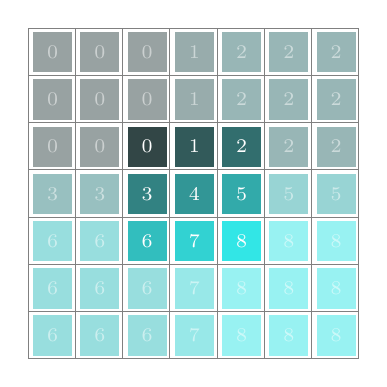
\begin{tikzpicture}[x  = {(1cm,0cm)},
    y  = {(0cm,1cm)},
    z  = {(-.5cm,-.5cm)},
    scale=.6]

  \scriptsize

  \draw [very thin, gray] (0,0) grid (7,7);


  \foreach \pos / \v in {(0,2)/0, (1,2)/1, (2,2)/2, (0,1)/3, (1,1)/4, (2,1)/5, (0,0)/6, (1,0)/7, (2,0)/8} {
      \pgfmathsetmacro{\hue}{70+20*\v} ;
      \draw (2.1,2.05) + \pos node[above right, inner sep=5px,color=white,fill={rgb,255:red,50;green,\hue;blue,\hue}] {\v} ;
    }

  \foreach \pos / \v in {(0,0)/6,(0,1)/6,(0,2)/6,(0,3)/3,(0,4)/0,(0,5)/0,(0,6)/0} {
      \pgfmathsetmacro{\hue}{70+20*\v} ;
      \draw (0.1,0.05) + \pos node[above right, inner sep=5px,color=white,opacity=0.5,fill={rgb,255:red,50;green,\hue;blue,\hue}] {\v} ;
    }

  \foreach \pos / \v in {(1,0)/6,(1,1)/6,(1,2)/6,(1,3)/3,(1,4)/0,(1,5)/0,(1,6)/0} {
      \pgfmathsetmacro{\hue}{70+20*\v} ;
      \draw (0.1,0.05) + \pos node[above right, inner sep=5px,color=white,opacity=0.5,fill={rgb,255:red,50;green,\hue;blue,\hue}] {\v} ;
    }

  \foreach \pos / \v in {(5,0)/8,(5,1)/8,(5,2)/8,(5,3)/5,(5,4)/2,(5,5)/2,(5,6)/2} {
      \pgfmathsetmacro{\hue}{70+20*\v} ;
      \draw (0.1,0.05) + \pos node[above right, inner sep=5px,color=white,opacity=0.5,fill={rgb,255:red,50;green,\hue;blue,\hue}] {\v} ;
    }

  \foreach \pos / \v in {(6,0)/8,(6,1)/8,(6,2)/8,(6,3)/5,(6,4)/2,(6,5)/2,(6,6)/2} {
      \pgfmathsetmacro{\hue}{70+20*\v} ;
      \draw (0.1,0.05) + \pos node[above right, inner sep=5px,color=white,opacity=0.5,fill={rgb,255:red,50;green,\hue;blue,\hue}] {\v} ;
    }

  \foreach \pos / \v in {(2,0)/6,(2,1)/6,(3,0)/7,(3,1)/7,(4,0)/8,(4,1)/8} {
      \pgfmathsetmacro{\hue}{70+20*\v} ;
      \draw (0.1,0.05) + \pos node[above right, inner sep=5px,color=white,opacity=0.5,fill={rgb,255:red,50;green,\hue;blue,\hue}] {\v} ;
    }

  \foreach \pos / \v in {(2,5)/0,(2,6)/0,(3,5)/1,(3,6)/1,(4,5)/2,(4,6)/2} {
      \pgfmathsetmacro{\hue}{70+20*\v} ;
      \draw (0.1,0.05) + \pos node[above right, inner sep=5px,color=white,opacity=0.5,fill={rgb,255:red,50;green,\hue;blue,\hue}] {\v} ;
    }

\end{tikzpicture}
\end{document}


